\chapter*{Supporting Information}

\makeatletter
\renewcommand{\fnum@figure}{\figurename~S\thefigure}
\makeatother

\makeatletter
\renewcommand{\fnum@table}{\tablename~S\thetable}
\makeatother

\setcounter{figure}{0}

% MSA Matrix :
\begin{figure}[H]
	\label{MSA + AF + AFi}
	\center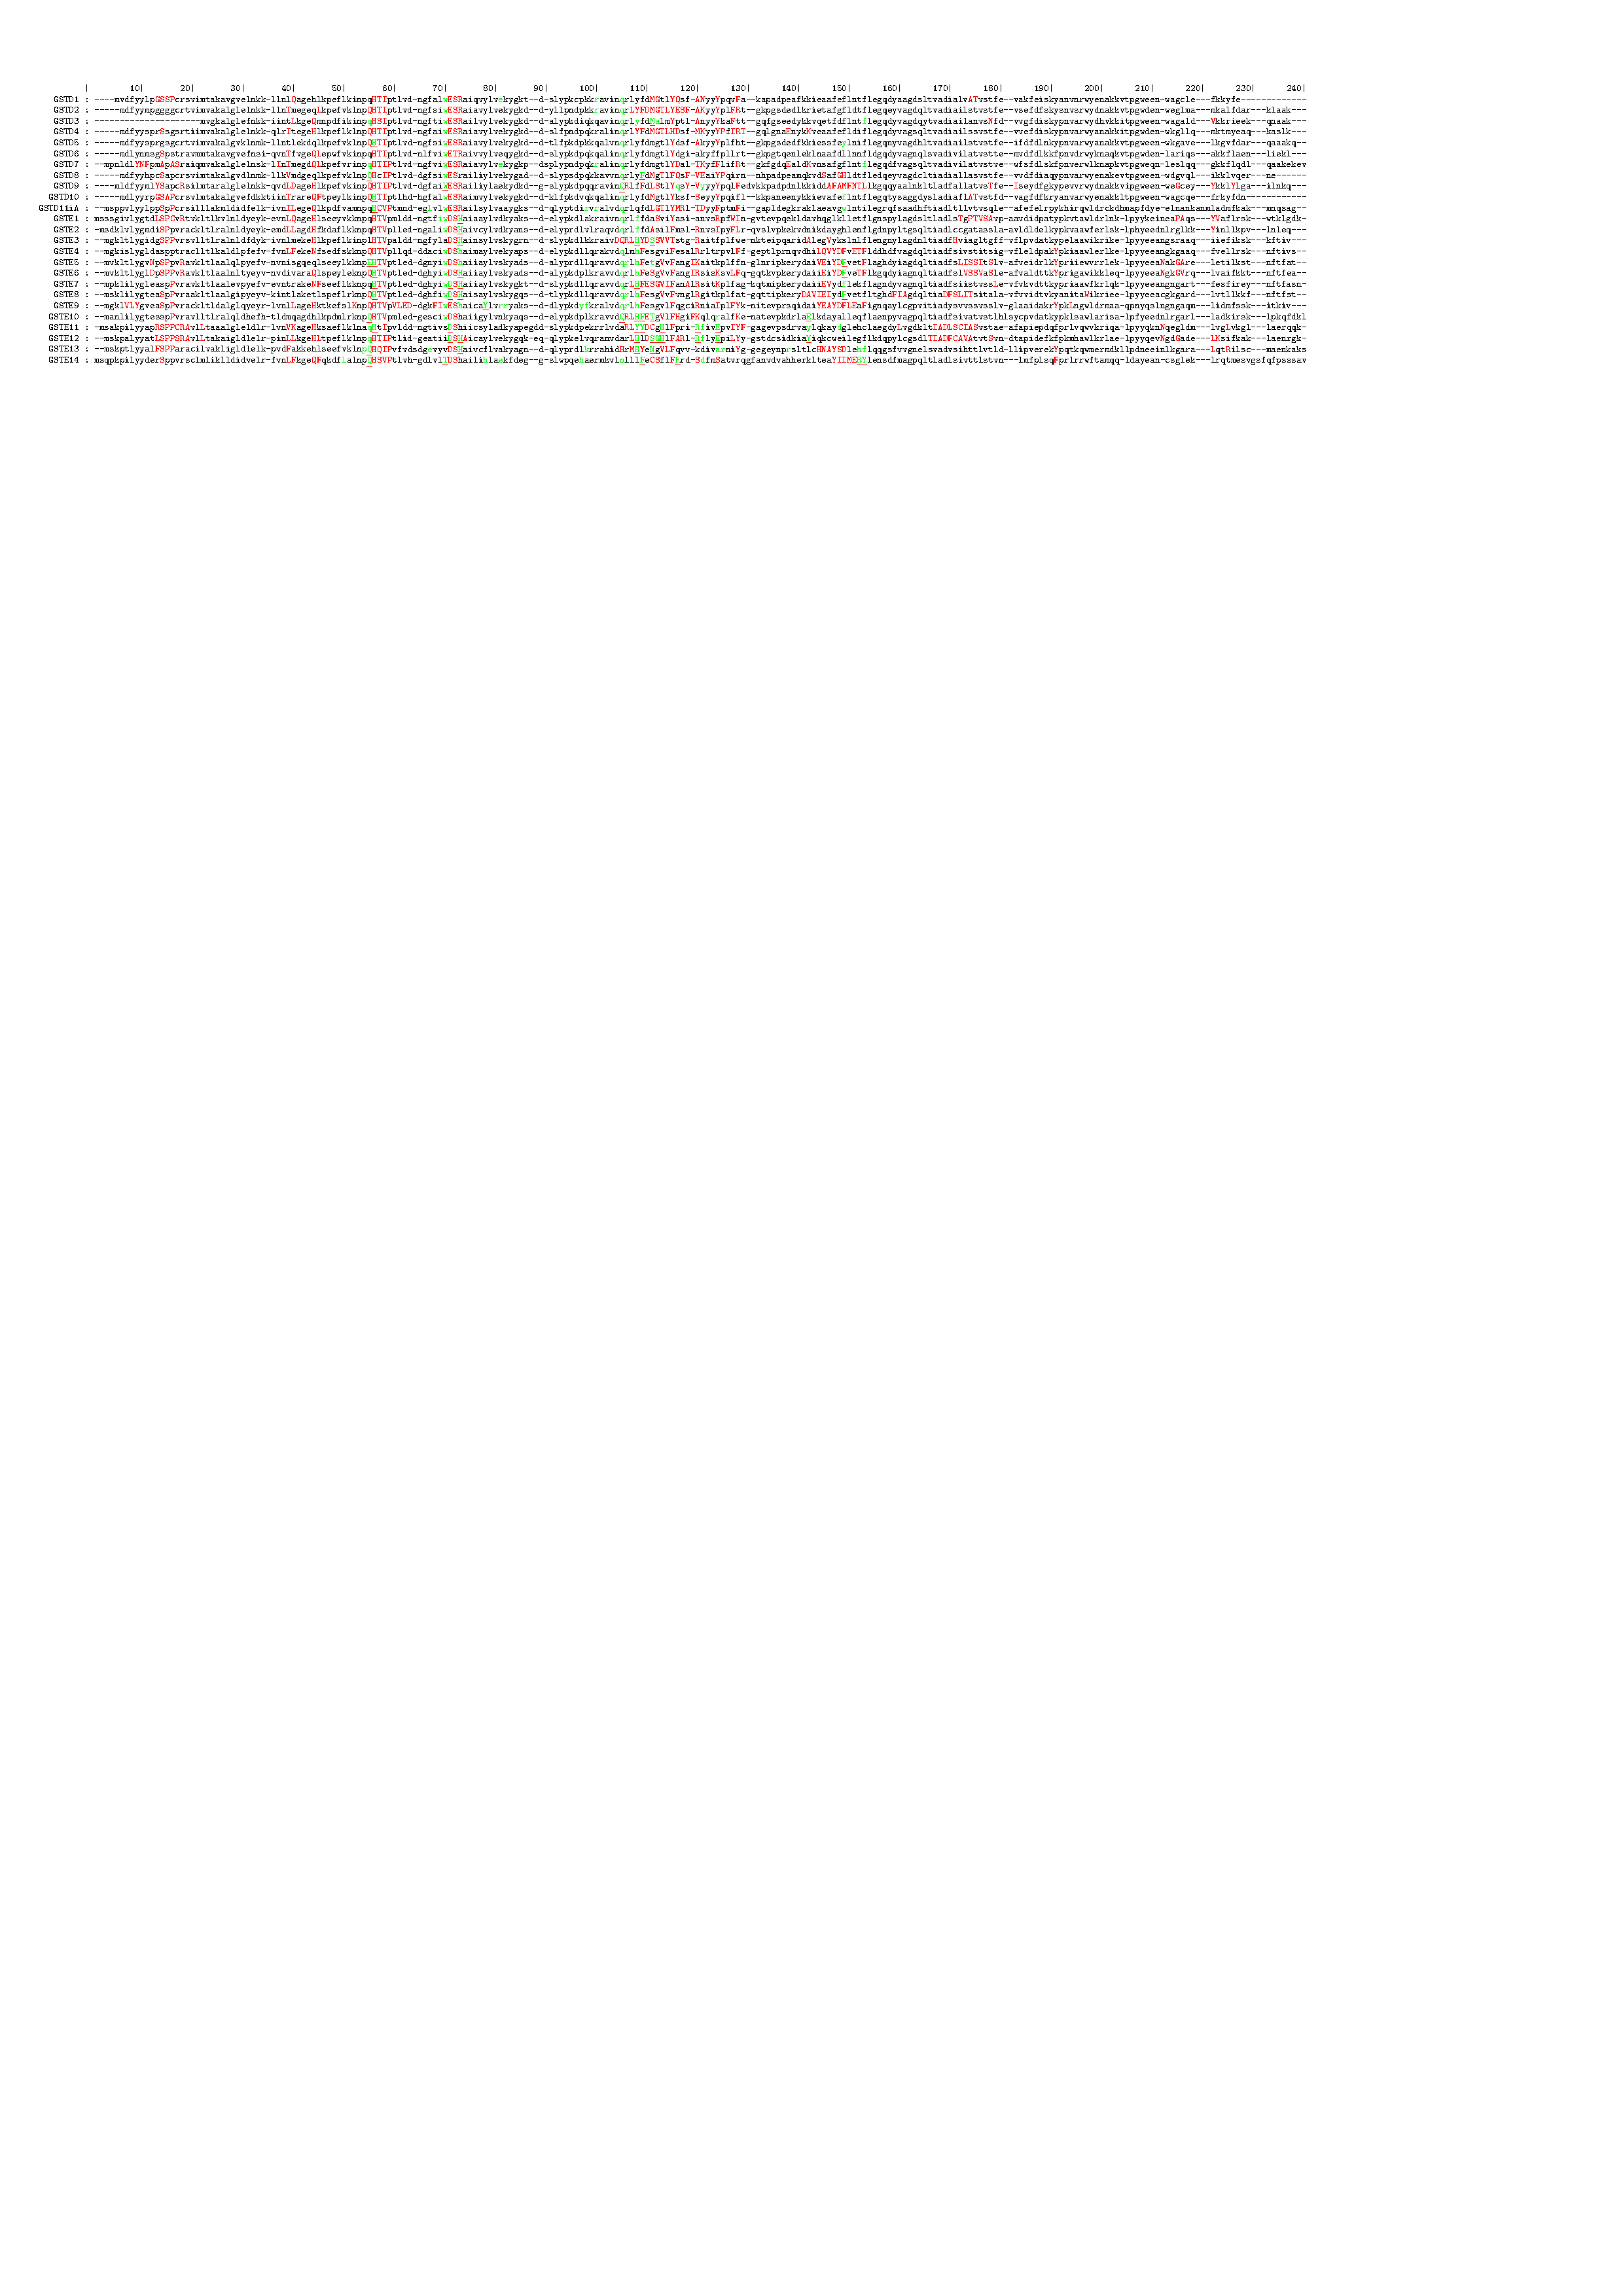
\includegraphics[width = .99\linewidth]{figures/MSA_matrix.pdf} % MSA + AF + AFi
	\caption{MSA matrix for the 25 considered GSTs with the predicted binding site (red residues) and dimer interface (green residues)}
\end{figure}
	
% Conservation in Binding sites :
\begin{figure}
	\label{Conservation BSs}
	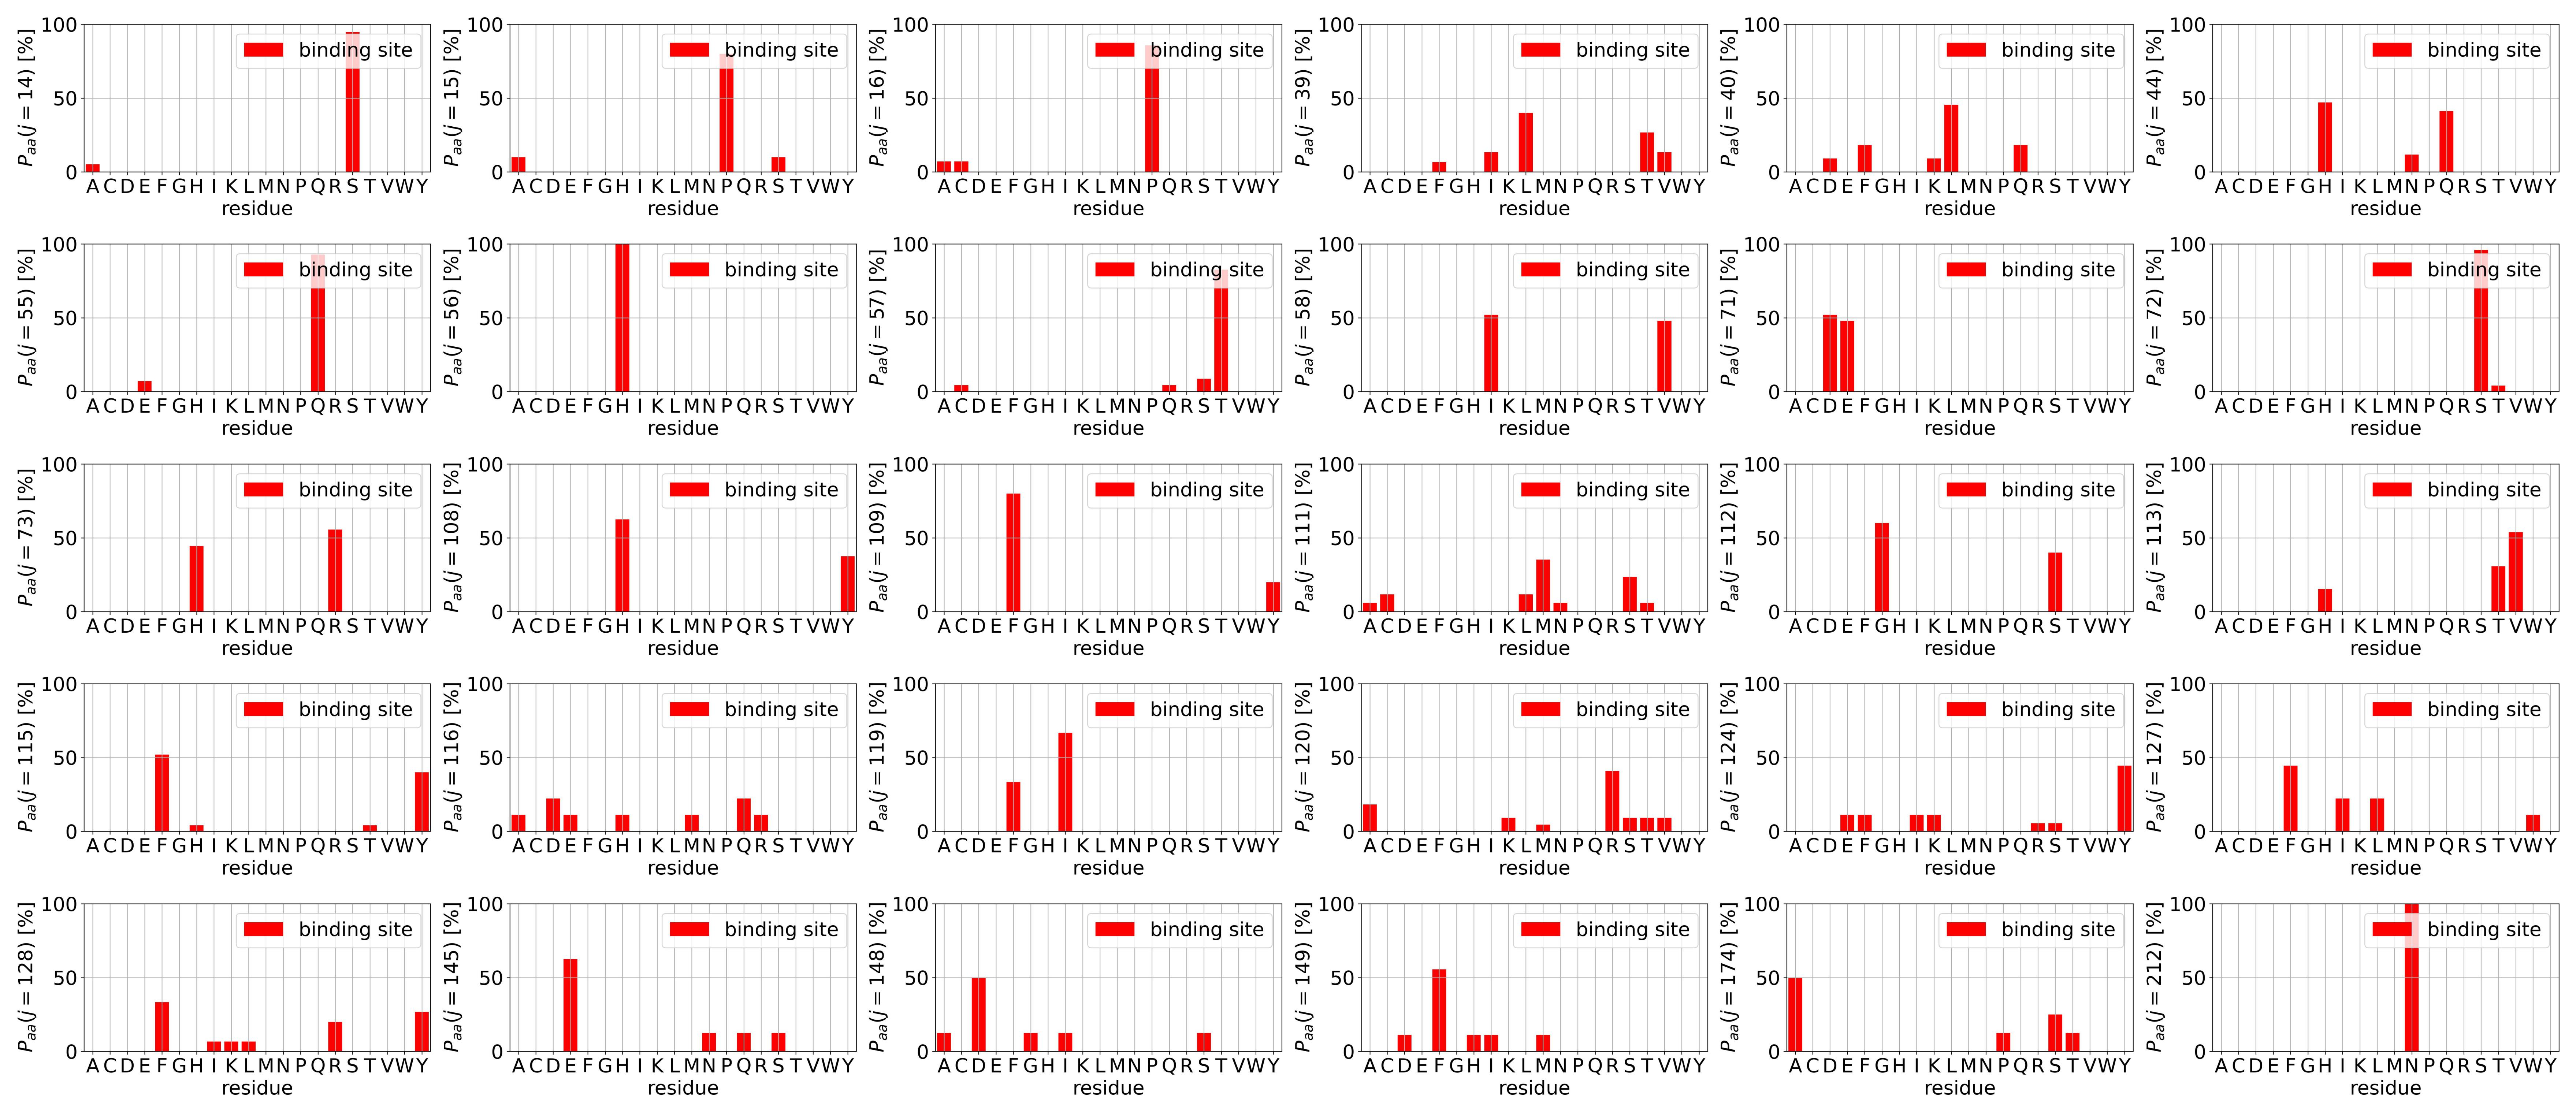
\includegraphics[width = .99\linewidth]{figures/Conservation_array_binding_site.jpg}
	\caption{Conservations of the amino-acids that have been identified as a part of the binding site}
\end{figure}

% Conservation in Dimer interfaces :
\begin{figure}
	\label{Conservation BSs}
	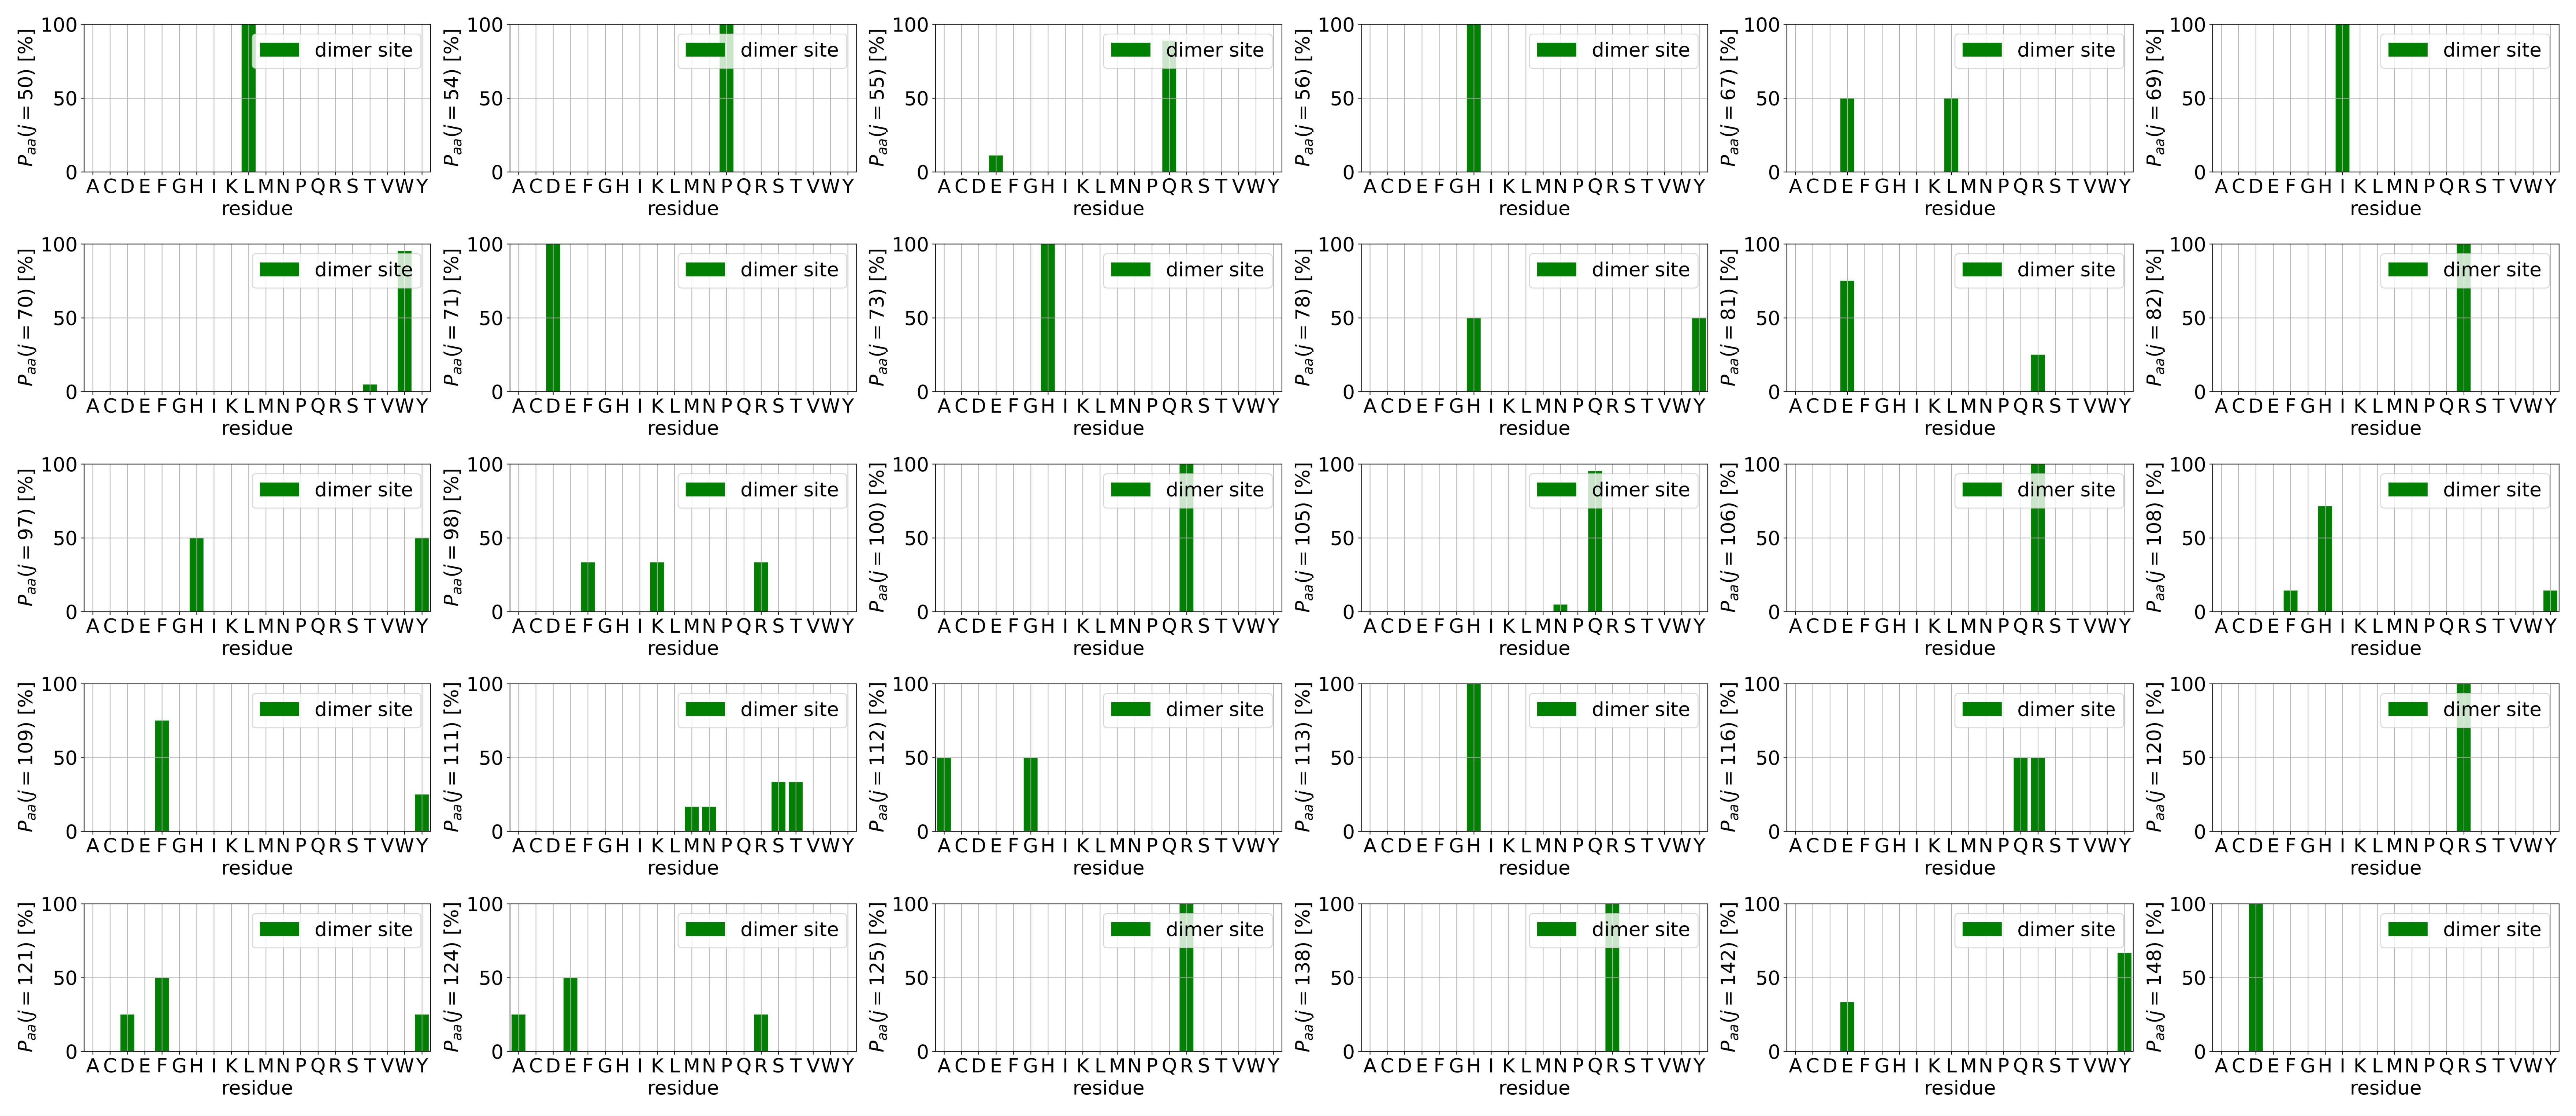
\includegraphics[width = .99\linewidth]{figures/Conservation_array_dimer_interface.jpg}
	\caption{Conservations of the amino-acids that have been identified as a part of the dimer interface}
\end{figure}